\chapter{Løsning}
\lhead{Løsning}

\section{Krav}
For å se kravlistene \ref{kravliste1} og \ref{kravliste2} 



Utifra denne kravlisten ble et workflow en bruker skal benytte ved bestilling av bil laget:
WORKFLOW!!

\subsection{Workflow}
En kunde skal kunne benytte nettsiden som et bestillingsverktøy. %Kunden skal selv ha kontroll på hvordan han finner frem til bilen som passer best. %Hovedsakelig skal man ha 2 alternativer: 
%Søke basert på dato i leieperioden og biltype, \textbf{eller} se en komplett liste over alle biler, evt. basert på kategori. 
\subsubsection{Fremgangsmåte}
\begin{steps}{Steg}
\step \textbf{Forside}\\Man starter med å se på forsiden av nettsiden. Denne skal inneholde generell informasjon om bedriften, litt om hvordan leien fungerer, priser, vilkår osv. Utover dette skal det her være 2 muligheter for kunden å gå videre i reservasjonsprosessen:\\
\textbf{Søke på Dato} Her skal systemet finne ut hvilke biler som er ledige i en leieperiode, og returnere disse. \\
\textbf{Se Biler} Man kan se alle bilene innenfor en gitt kategori, eller alle biler i systemet.

\step \textbf{Liste over biler}\\Uavhengig av fremgangsmåten kunden har valgt, vil man nå presenteres med en liste over biler. Listen inneholder generell informasjon om hver av bilene, samt bilde og døgnpris i leien.\\
Utifra denne listen velger kunden å gå videre på en av bilene.

\step \textbf{Spesifikk bil}\\Nå befinner kunden seg på siden til den bestemte bilen. Her skal informasjon om bilen og eventuelle bilder presenteres.
Dersom kunden ikke søkte på dato i Steg 1, må det her sjekkes når bilen er ledig for utleie. Dette skal visualiseres i form av en kalender.\\
Videre skal kunden fylle inn dato i leieperioden (Dersom man søker på Dato i Steg 1, skal dette bli fylt inn automatisk), så gå videre.

\step \textbf{Kontakt Informasjon}\\Det siste steget av reservasjonsprosessen. Her skal kunden fylle inn kontakt informasjon, og kunne se informasjon om reservasjonen og den valgte bil.\\
Når informasjonen er fylt inn trykker brukeren på Fullfør Bestilling, som skal videreføre til en bekreftelses side om hele bestillingen. Nå skal også en epost bli sendt til kunden som inneholder nødvendig informasjon om bestillingen.

\step \textbf{Last ned informasjon som PDF (Valgfritt)}\\Brukeren skal ha mulighet til å laste ned ordre bekreftelse som PDF 

\end{steps}




\section{Designspesifikasjoner}
%Sette Workflow her?

\newpage
\section{Nettsiden}
\subsection{Design}
\subsubsection{Forsiden}
 \begin{figure}[htbp]
	\centering
		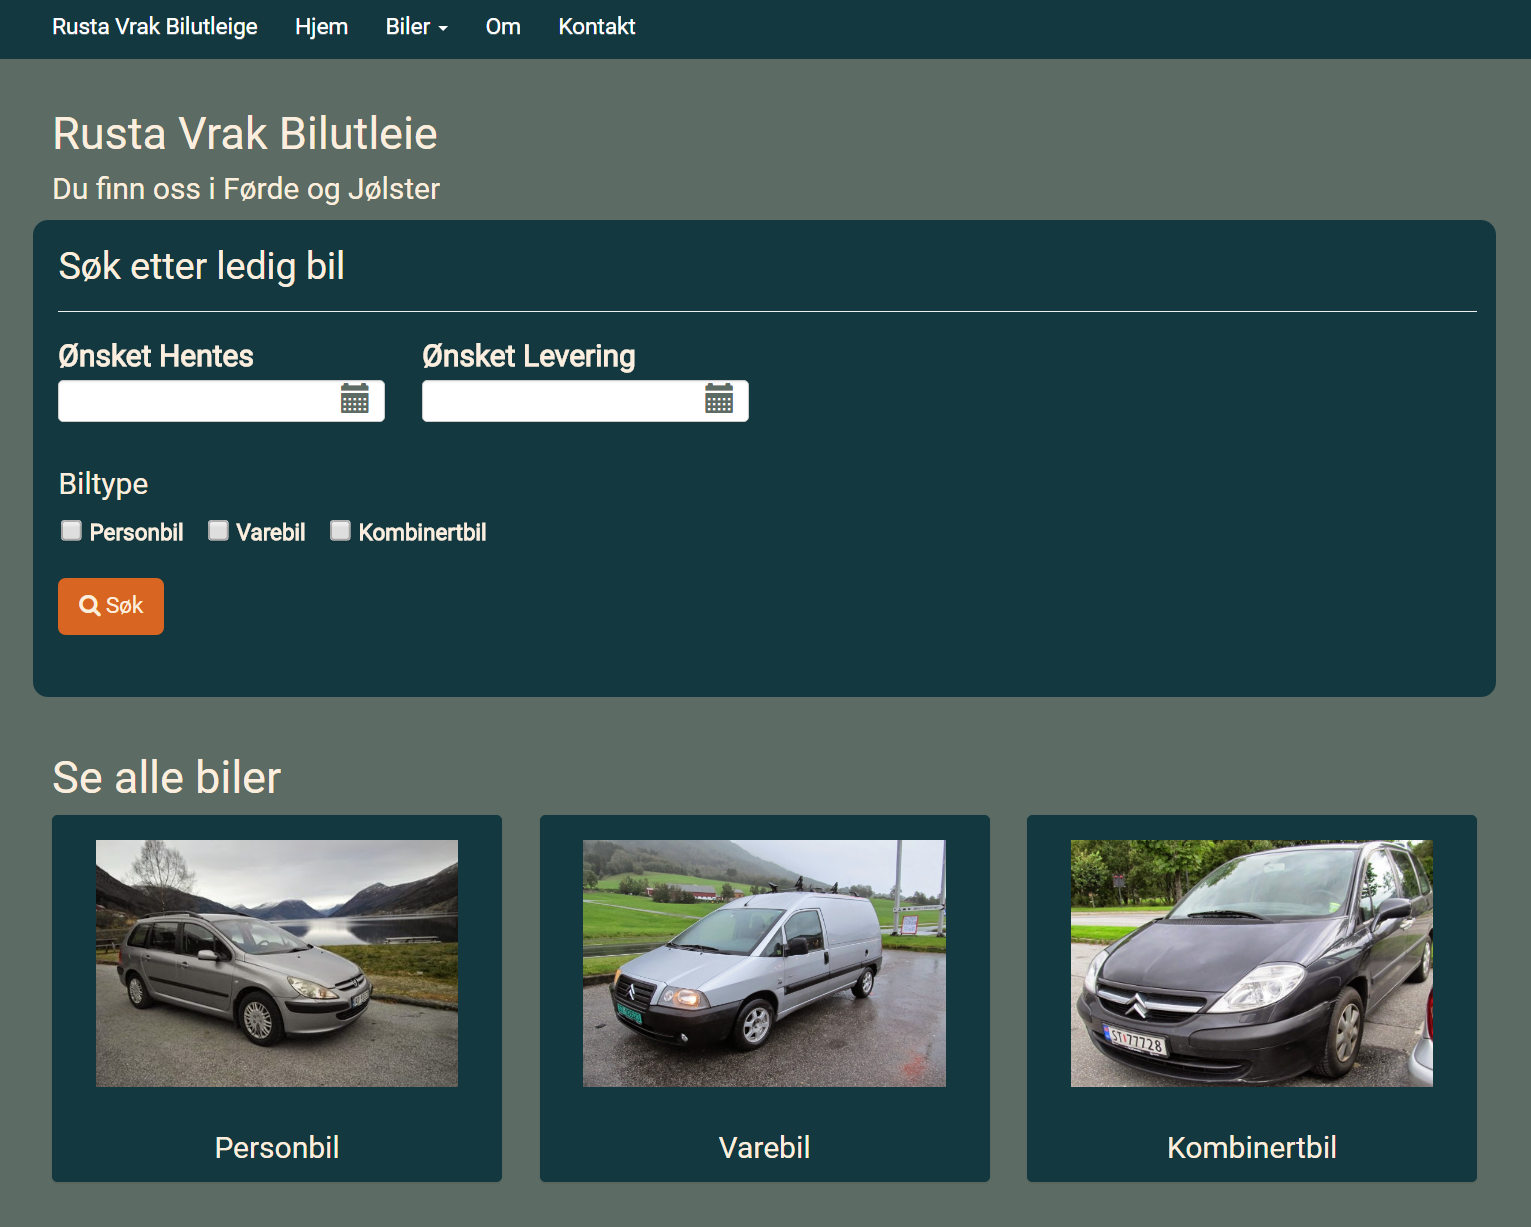
\includegraphics[scale=0.3]{Bilder/rv_frontpage.png}
	\caption[Utleiepris Diagram]{Oversikt over rabatt som tilføres i forhold til hvor lenge en bil blir utleid. } %\ref{fig:iterative}
	\label{fig:rv_frontpage}
\end{figure}


\subsubsection{Bil Liste}
 \begin{figure}[htbp]
	\centering
		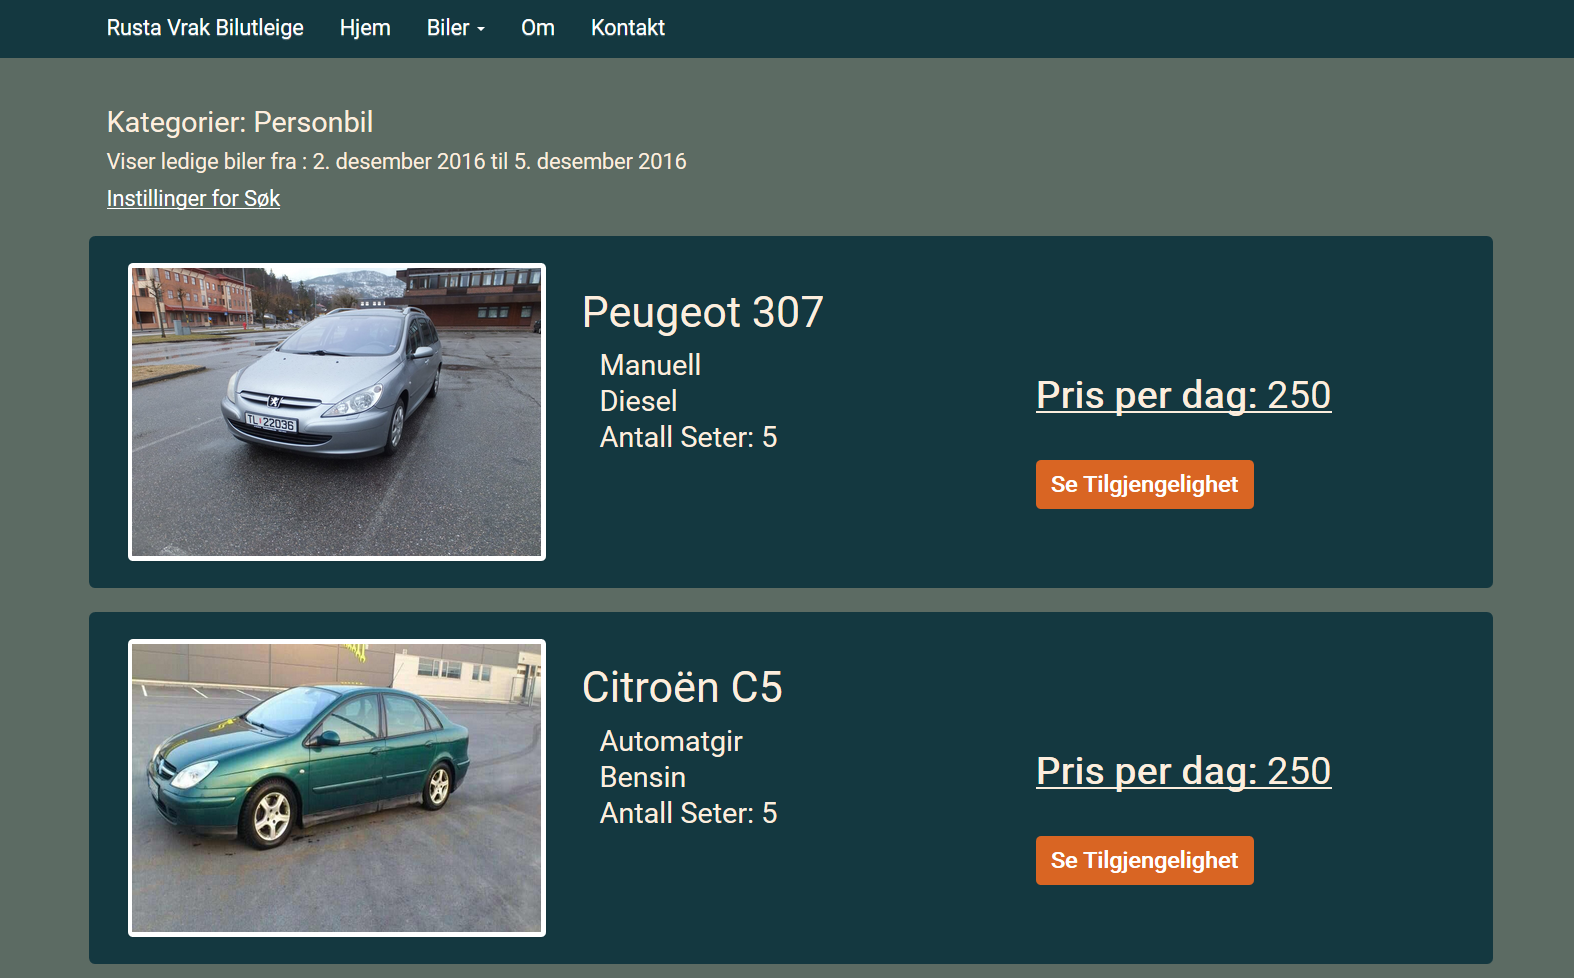
\includegraphics[scale=0.3]{Bilder/rv_carlist.png}
	\caption[Utleiepris Diagram]{Oversikt over rabatt som tilføres i forhold til hvor lenge en bil blir utleid. } %\ref{fig:iterative}
	\label{fig:rv_carlist}
\end{figure}

\subsubsection{Individuelle Biler}
 \begin{figure}[htbp]
	\centering
		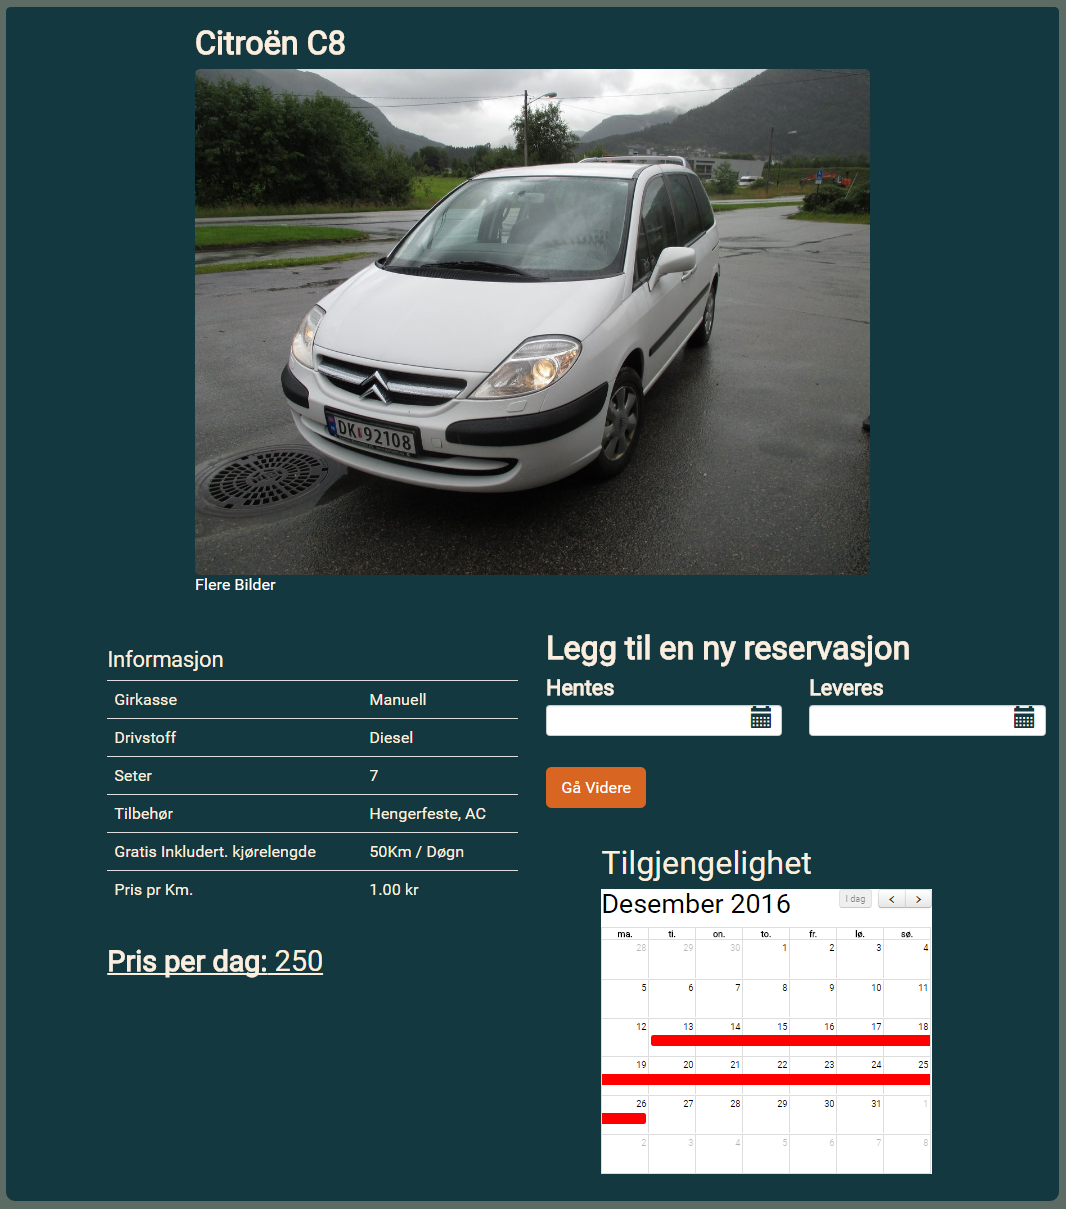
\includegraphics[scale=0.3]{Bilder/rv_individualcar.png}
	\caption[Utleiepris Diagram]{Oversikt over rabatt som tilføres i forhold til hvor lenge en bil blir utleid. } %\ref{fig:iterative}
	\label{fig:rv_individualcar}
\end{figure}


 \begin{figure}[htbp]
	\centering
		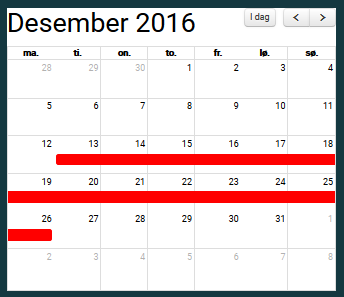
\includegraphics[scale=0.3]{Bilder/rv_dateavailable.png}
	\caption[Utleiepris Diagram]{Oversikt over rabatt som tilføres i forhold til hvor lenge en bil blir utleid. } %\ref{fig:iterative}
	\label{fig:rv_dateavailable}
\end{figure}



\subsubsection{Kontakt Informasjon}
 \begin{figure}[htbp]
	\centering
		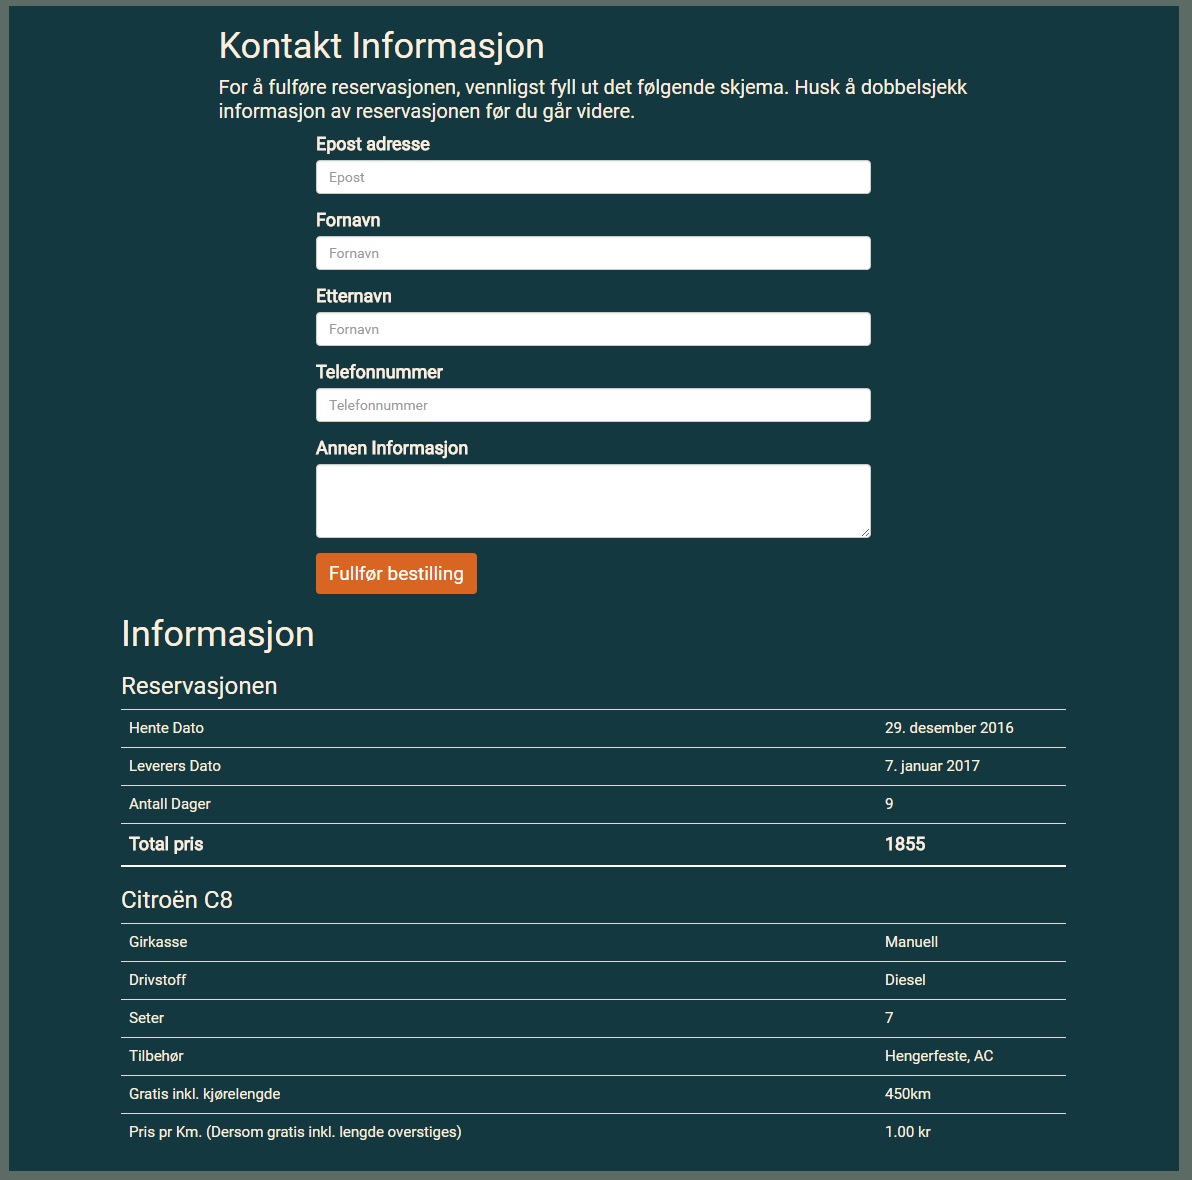
\includegraphics[scale=0.3]{Bilder/rv_customercontact.png}
	\caption[Utleiepris Diagram]{Oversikt over rabatt som tilføres i forhold til hvor lenge en bil blir utleid. } %\ref{fig:iterative}
	\label{fig:rv_customercontact}
\end{figure}

\subsubsection{Kvittering}






\clearpage
\section{Administrasjon Side}
Administrasjonssiden skal hovedsakelig benyttes av bedriften for å kunne holde et styr over sine biler og bestillinger. På figur \ref{fig:admin_front} kan man se et skjermbilde av forsiden av admin siden. Denne admin siden blir generert av Django og reflekterer de konfigurasjonene som blir gjort i koden. Man velger bl.a. hvilke tabeller som er interessante å ha i admin siden, hvilke elementer som skal ligge i listen, søke funksjoner osv. Her har man også muligheten til å opprette nye admin kontoer og velge hvilke rettigheter de skal kunne ha på nettsiden.

 \begin{figure}[htbp]
	\centering
		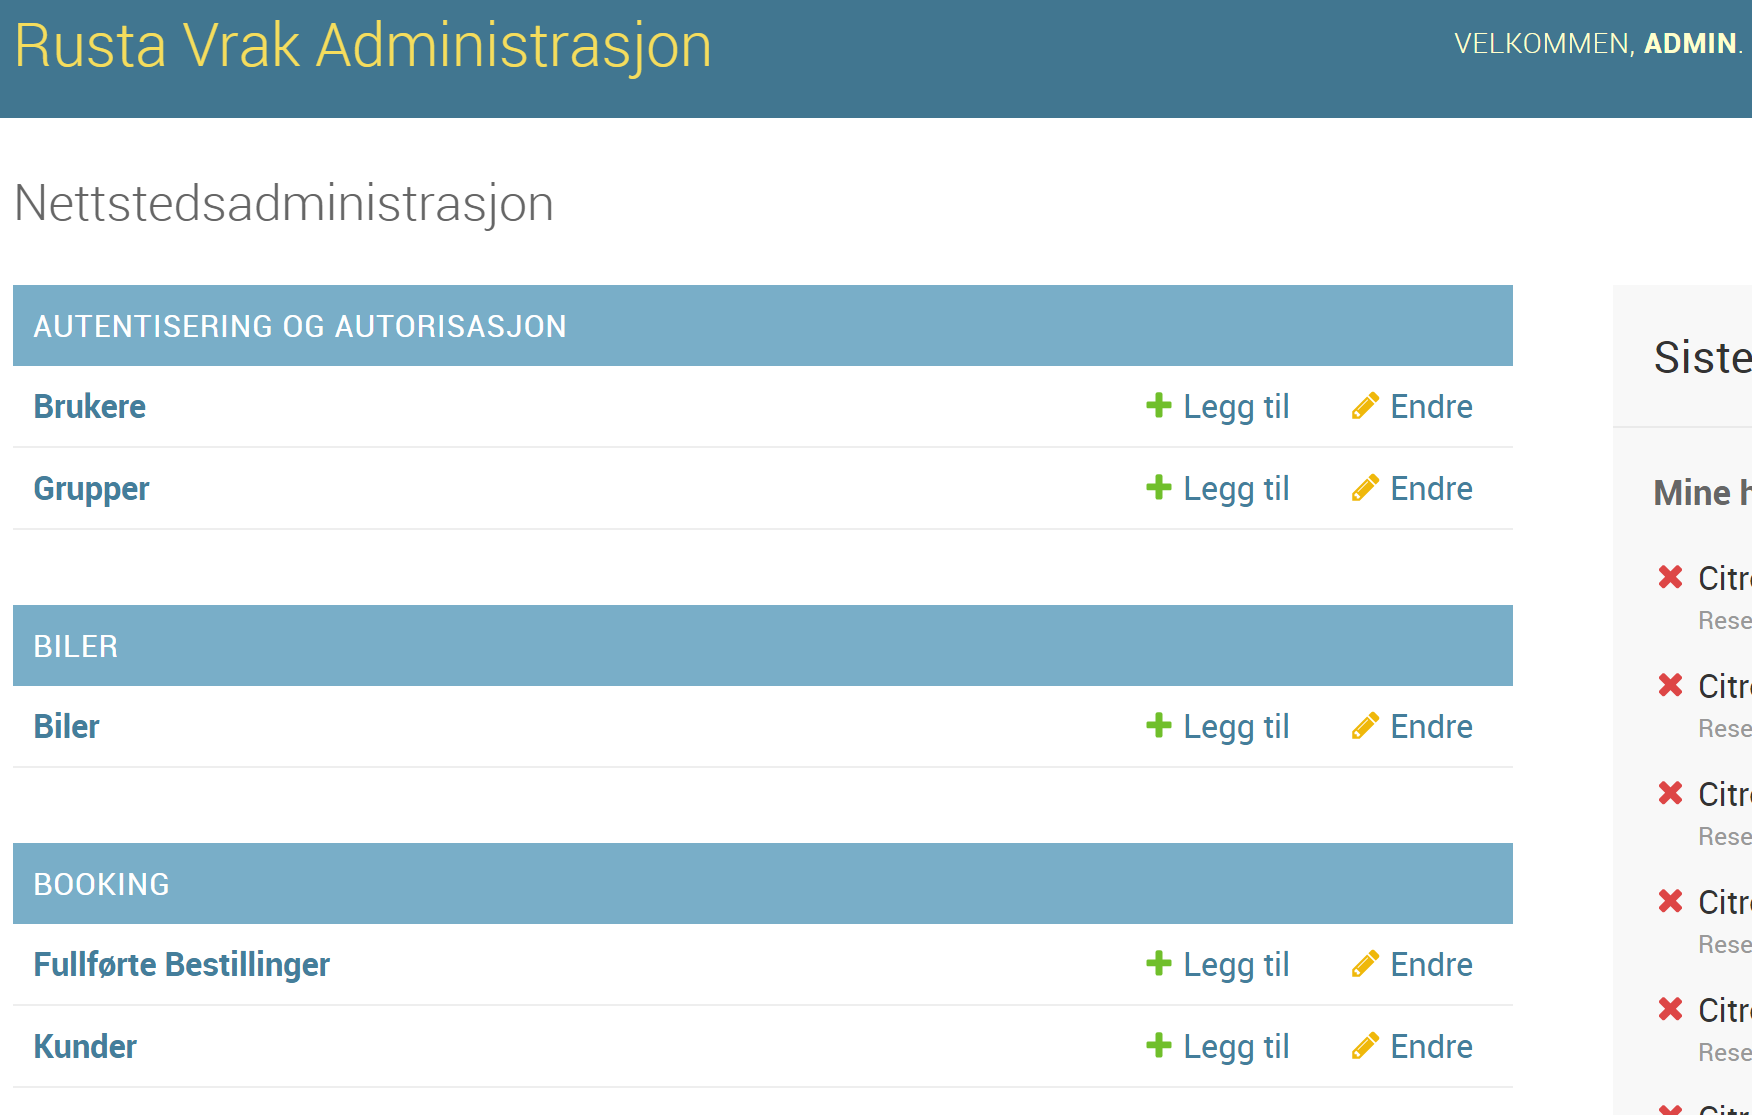
\includegraphics[scale=0.3]{Bilder/admin_forside.png}
	\caption[Forside i Administrasjons Side]{Hvordan administrasjonssiden ser ut. Denne har blitt generert og konfigurert med Django. } %\ref{fig:iterative}
	\label{fig:admin_front}
\end{figure}
\newpage
\subsection{Reservasjoner i Administrasjonsside}
På figur \ref{fig:admin_list} kan man se listen over alle ferdig reservasjoner. Her kan man se informasjon om kunden, hvilken bil som er reservert, bestillings, hente og leveringsdato, og den totale prisen for reservasjonen. \\
For å kunne filtrere ut spesifikke reservasjonen kan man bruke søke funksjonen. Denne godtar søk på skiltnummer, bilmerke og modell, kundens etternavn og epost. Søket blir gjort å en såkalt «Contains» metode, som betyr at dersom man f.eks. gjør et søk på ‘TV’, vil reservasjonen med en bil med skiltnummer ‘TV65282’ bli med i resultatet.

 \begin{figure}[htbp]
	\centering
		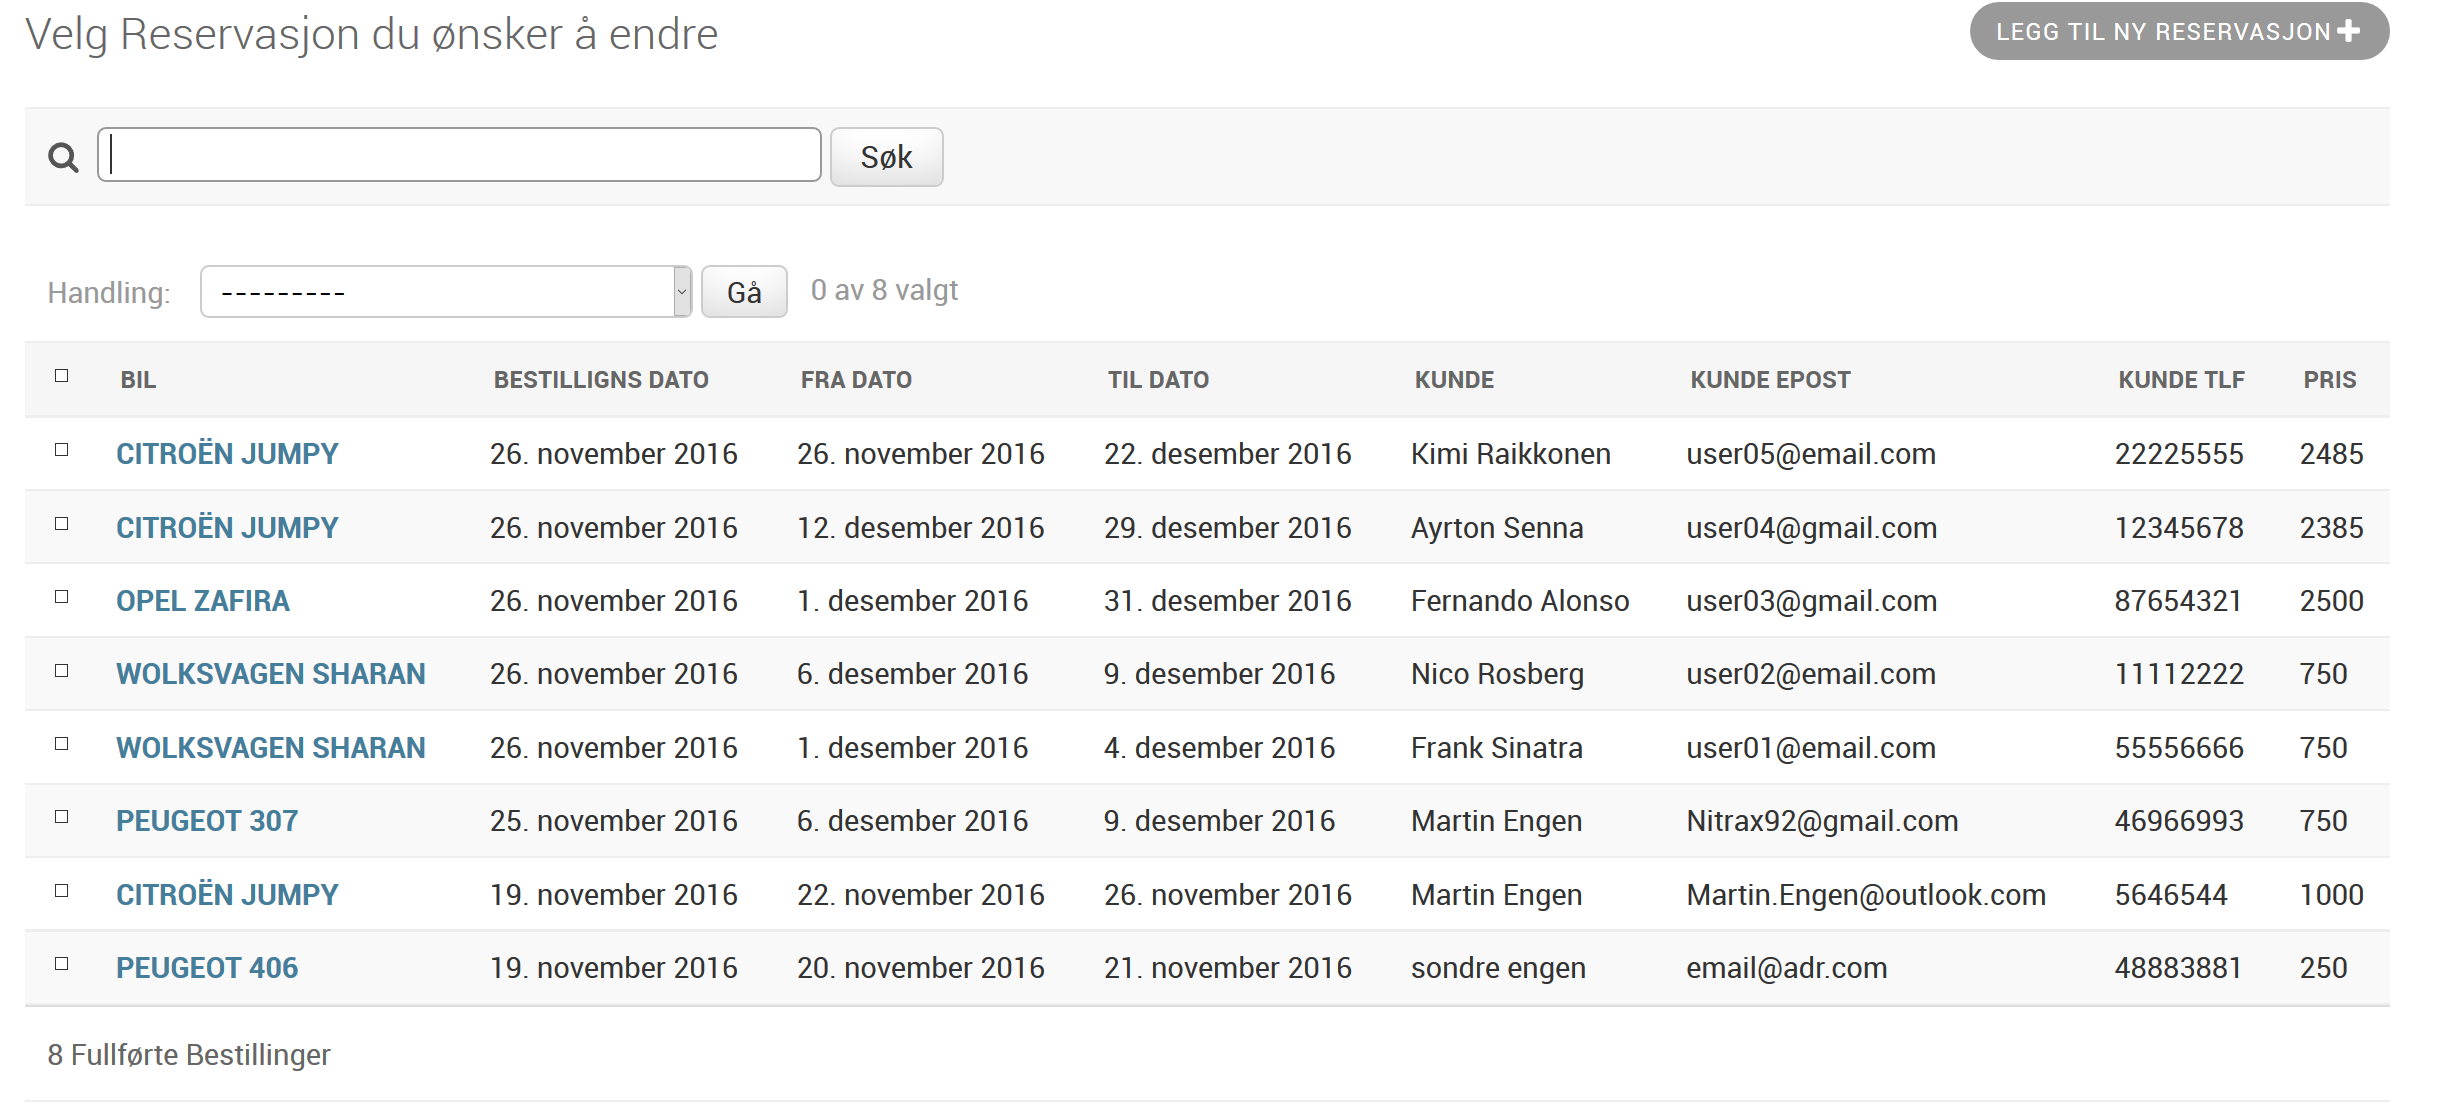
\includegraphics[width=16cm, keepaspectratio]{Bilder/admin_liste2.png}
	\caption[Administrasjonsside - Oversikt over reservasjoner]{Liste over alle reservasjoner registert på nettsiden. } %\ref{fig:iterative}
	\label{fig:admin_list}
\end{figure}





\subsubsection*{Legge til ny reservasjon}




\begin{figure}[h!]
\begin{flushright}
\begin{minipage}{0.4\textwidth}
\begin{center}
    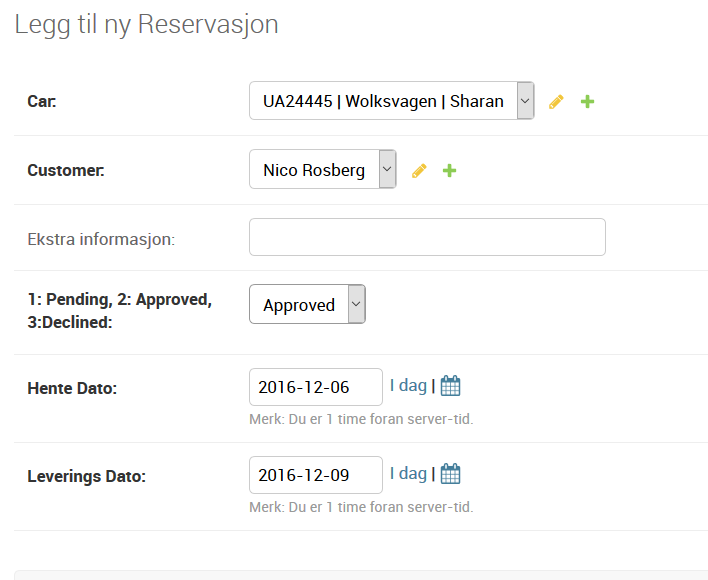
\includegraphics[width=1.2\textwidth]{Bilder/admin_ny_reservasjon.png}
    \caption{Gripper}
    \label{fig:admin_new_res}
\end{center}
\end{minipage}
\end{flushright}
\end{figure}


%
\vspace{-7cm}
%
\begin{flushleft}
\begin{minipage}{0.5\textwidth}

%
%
Dersom en kunde ikke ønsker å reservere gjennom nettsiden, kan ansatte også gjøre dette gjennom administrasjons siden. Som beskrevet i Workflow seksjonen, er det en enkel prosess. Man velger å legge til en ny reservasjon, fyller ut vinduet (Se Figur \ref{fig:admin_new_res}) og lagrer dette.

\end{minipage}
\end{flushleft}

\newpage
\section{Priser og Rabatt}
Rusta Vrak Bilutleige ønsker at når en kunde først skal leie en bil, skal det være så lenge som mulig for å slippe å hente og levere biler mer enn nødvendig. Derfor vil bedriften gi kunder gode rabatter som øker i forhold til lenge på leieperiode. Leieprisen av de aller fleste bilene ligger på 250kr pr. døgn, og i dag tilbyr bedriften utleie for 30 dager for kun 2500kr. Dette tilsvarer en prisreduksjon på 66.6\%. For å kunne implementere et liknende system på nettsiden ble det laget en rekke løsningsforslag i Excel, dette finner man vedlagt i vedlegg OOAWNDO

\subsection*{Valgte Løsning}
Den valgte løsningen går ut på å gi kunden 17.5\% ekstra avslag hver 5. dag i leieperioden. Se tabell \ref{table:percent} for en oversikt over hvordan pris avslaget stiger. Figur \ref{fig:price_reduction} viser hvordan prisantydningen blir på biler som har en døgnpris på 250kr. Dette vil kunne bidra til at en kunde leier litt ekstra kun for å få ekstra avslag på prisen. 

\begin{table}[htbp]
\centering
\caption{Rabatt man oppnår ved leieperioder}
\label{table:percent}
\begin{tabular}{|l|l|l|l|l|l|l|l|l}
\cline{1-8}
Antall Dager & 0-4   & 5-9    & 10-14     & 15-19    & 20-24    & 25-29    & 30      &  \\ \cline{1-8}
Rabatt       & 100\% & 82.5\% & 68.0625\% & 56.151\% & 46.325\% & 38.218\% & 33.33\% &  \\ \cline{1-8}
\end{tabular}
\end{table}



 \begin{figure}[htbp]
	\centering
		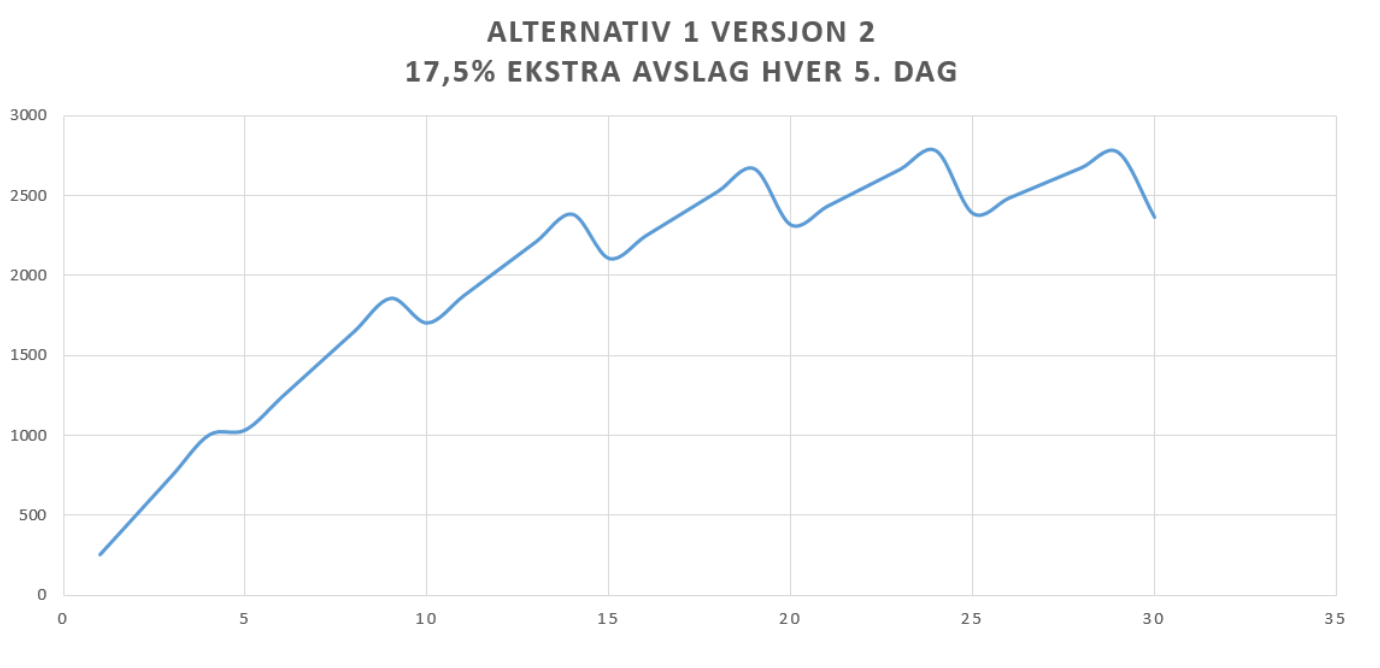
\includegraphics[scale=0.5]{Bilder/avslag.png}
	\caption[Utleiepris Diagram]{Oversikt over rabatt som tilføres i forhold til hvor lenge en bil blir utleid. } %\ref{fig:iterative}
	\label{fig:price_reduction}
\end{figure}








\clearpage
\section{Database}
Dette prosjektet benytter Django, og dermed vil dette rammeverket ta hånd om mye av arbeidet mot databasen. Django kommer utstyrt med en ORM (Object Relational Mapper), som håndterer overgangen fra Python klasseer til MySQL tabeller. 

\clearpage
\section{Testing og Validering}
Det har blitt benyttet en iterativ arbeidsmetode som beskrevet tidligere: [REF BESKREVET METODE]. Denne metoden tilsier at testing skal og må foregå underveis i utviklingen i hver syklus. Dette har blitt gjennomført vha. pythons logging bibliotek og Djangos debuggings modus. 


